\documentclass[a4paper, 12pt]{report}
\usepackage{cmap}
\usepackage{amssymb}
\usepackage{amsmath}
\usepackage{graphicx}
\usepackage{amsthm}
\usepackage{upgreek}
\usepackage{setspace}
\usepackage{color}
\usepackage{moreverb}
\usepackage[T2A]{fontenc}
\usepackage[utf8]{inputenc}
\usepackage[normalem]{ulem}
\usepackage{mathtext} % русские буквы в формулах
\usepackage[left=2cm,right=2cm, top=2cm,bottom=2cm,bindingoffset=0cm]{geometry}
\usepackage[english,russian]{babel}
\usepackage[unicode]{hyperref}
\newenvironment{Proof} % имя окружения
{\par\noindent{$\blacklozenge$}} % команды для \begin
{\hfill$\scriptstyle\boxtimes$}
\newcommand{\Rm}{\mathbb{R}}
\newcommand{\Cm}{\mathbb{C}}
\newcommand{\Z}{\mathbb{Z}}
\newcommand{\I}{\mathbb{I}}
\newcommand{\N}{\mathbb{N}}
\newcommand{\rank}{\operatorname{rank}}
\newcommand{\Ra}{\Rightarrow}
\newcommand{\ra}{\rightarrow}
\newcommand{\FI}{\Phi}
\newcommand{\Sp}{\text{Sp}}
\renewcommand{\leq}{\leqslant}
\renewcommand{\geq}{\geqslant}
\renewcommand{\alpha}{\upalpha}
\renewcommand{\beta}{\upbeta}
\renewcommand{\gamma}{\upgamma}
\renewcommand{\delta}{\updelta}
\renewcommand{\varphi}{\upvarphi}
\renewcommand{\phi}{\upvarphi}
\renewcommand{\tau}{\uptau}
\renewcommand{\lambda}{\uplambda}
\renewcommand{\psi}{\uppsi}
\renewcommand{\mu}{\upmu}
\renewcommand{\omega}{\upomega}
\renewcommand{\d}{\partial}
\renewcommand{\xi}{\upxi}
\renewcommand{\epsilon}{\upvarepsilon}
\newcommand{\intx}{\int\limits_{x_0}^x}
\newcommand\Norm[1]{\left\| #1 \right\|}
\newcommand{\sumk}{\sum\limits_{k=0}^\infty}
\newcommand{\sumi}{\sum\limits_{i=0}^\infty}
\newtheorem*{theorem}{Теорема}
\newtheorem*{cor}{Следствие}
\newtheorem*{lem}{Лемма}
\begin{document}
	% Оформление титульного листа
	\begin{titlepage}
		\begin{center}
			\textsc{МИНИСТЕРСТВО ОБРАЗОВАНИЯ РЕСПУБЛИКИ БЕЛАРУСЬ БЕЛОРУССКИЙ ГОСУДАРСТВЕННЫЙ УНИВЕРСИТЕТ
				\\[5mm]
				ФАКУЛЬТЕТ ПРИКЛАДНОЙ МАТЕМАТИКИ И ИНФОРМАТИКИ\\[2mm]
				Кафедра компьютерных технологий и систем
			}
			
			\vfill
			
			\textbf{Отчет по лабораторной работе №2\\
				«Решение смешанных задач для уравнения теплопроводности»\\
				Вариант 2
				\\[26mm]
			}
		\end{center}
		
		\hfill
		\begin{minipage}{.5\textwidth}
			\begin{flushright}
				Бовта Тимофея Анатольевича\\
				студента 3 курса\\
				специальности «прикладная математика»\\[5mm]
				
				Преподаватель:\\[2mm] 
				И. С. Козловская\\
			\end{flushright}
		\end{minipage}%
		\vfill
		\begin{center}
			Минск, 2024\ г.
		\end{center}
	\end{titlepage}
	\newpage
	\section*{Постановка задачи}
	Решить следующую смешанную задачу $$\begin{cases}
		u_t - a^2 u_{xx} = \cos\dfrac{2\pi}{l}x,\\
		u_x|_{x=0} = 0,\\
		u_x|_{x=l} = 0,\\
		u|_{t=0} = \cos\dfrac{2\pi}{l}x.
	\end{cases}$$
	\section*{Решение задачи аналитически}
	По методу разделения переменных для решения смешанных задач мы будем искать решение данной задачи в виде суммы 
	\begin{eqnarray}
		u(x,t) = \sum_{k=0}^{\infty} T_k(t)X_k(t),
	\end{eqnarray}
	где $X_k(t)$ --- это собственные функции соответствующей задачи Штурма-Лиувилля в предположении, что уравнение однородное.
	\subsubsection*{Решение задачи Штурма-Ливувилля}
	Пусть мы решаем соответствующую задачу для однородного уравнения. Тогда по методу разделения переменных мы получаем задачу Штурма-Лиувилля \begin{eqnarray}
	\begin{cases}
	X''(x) + \lambda X(x) = 0,\\
	X'(0) = 0,\\
	X'(l) = 0.
	\end{cases}
	\end{eqnarray}
	Задача (2) поставлена для линейного стационарного обыкновенного дифференциального уравнения (ОДУ) второго порядка, поэтому для ее решения будем строить соответствующее характеристическое уравнение $$\nu^2 + \lambda = 0.$$
	Считая $\lambda >0$, получаем $$\nu_{1,2} = \pm i\sqrt \lambda.$$
	Тогда общее решение для уравнения из задачи (2) имеет вид 
	\begin{eqnarray}
		X(x) = A\cos \sqrt \lambda x + B \sin \sqrt \lambda x.
	\end{eqnarray}
	Подставим граничные условия задачи (2) в данное решение. Для этого вычислим производную от функции $X(x)$:
	$$X'(x) = -A\sqrt \lambda \sin \sqrt \lambda x + B \sqrt \lambda \cos \sqrt \lambda x.$$
	Тогда для первого условия 
	$$X'(0) = B\sqrt \lambda = 0.$$
	Поскольку считаем $\lambda > 0$, то $B = 0$. Для второго условия, учитывая $B = 0$, имеем
	$$X'(l) = -A\sqrt \lambda \sin \sqrt \lambda l = 0.$$
	Тривиальное решение данной задачи нас не интересует, поэтому $A \ne 0$. Также $\lambda \ne 0$, а значит $$\sin \sqrt \lambda l =0.$$
	Отсюда $$\sqrt \lambda l = \pi k, \quad k =0,1,\ldots$$
	Таким образом, получаем, что собственные значения для оператора Штурма-Лиувилля равны $$\lambda_k = \left(\dfrac{\pi k}{l}\right)^2,\quad k = 0,1,\ldots.$$
	А отсюда можем построить собственные функции для этого оператора, которые и являются решениями поставленной задачи. Для этого подставим все найденные значения в общее решение (3) и получим $$X_k(x) = A \cos \dfrac{\pi k}{l} x.$$
	Поскольку собственные функции для каждого собственного значения определены с точностью до постоянного множителя, то для упрощения дальнейших вычислений примем $A = 1$. Таким образом, из задачи Штурма-Лиувилля мы имеем собственные значения и соответствующие им собственные функции вида 
	\begin{eqnarray}
	\lambda_k = \left(\dfrac{\pi k}{l}\right)^2,\quad X_k(x) = \cos \dfrac{\pi k}{l} x,\quad k = 0,1,\ldots.
	\end{eqnarray}
	\subsubsection*{Построение решения поставленной задачи}
	Итак, подставляя найденное значение $X_k(x)$ в общий вид решения (1), мы получаем $$u(x,t) = \sum_{k=0}^{\infty} T_k(t)  \cos \dfrac{\pi k}{l} x.$$ Чтобы определить вид функций $T_k(t)$, подставим данный вид решения в уравнение исходной задачи:
	$$\sum_{k=0}^\infty T'_k(t) \cos \dfrac{\pi k}{l}x + a^2 \sum_{k=0}^\infty T_k(t) \left(\dfrac{\pi k}{l}\right)^2 \cos \dfrac{\pi k}{l}x = \cos \dfrac{2\pi}{l}x.$$
	Преобразуем левую часть уравнения
	$$\sum_{k=0}^\infty\left( T'_k(t)  + \left(\dfrac{a\pi k}{l}\right)^2 T_k(t) \right) \cos \dfrac{\pi k}{l}x = \cos \dfrac{2\pi}{l}x.$$
	Итак, рассмотрим получившееся равенство. Слева мы имеем сумму, причем она является разложением в ряд Фурье по собственным функциям. Функцию с правой стороны равенства мы можем также разложить в ряд Фурье по собственным функциям вида $$\cos \dfrac{2\pi}{l}x = \sum_{k=0}^{\infty} \phi_k \cos \dfrac{k\pi}{l}x,\quad \phi_k = \begin{cases}
		1, \ k = 2,\\
		0, \ k \ne 2.
	\end{cases}$$
	Поскольку ряды равны, то их соответствующие коэффициенты совпадают. Тогда приравняем коэффициенты ряда слева к коэффициентам ряда справа и получим систему уравнений вида
	\begin{eqnarray}
		T'_2(t)  + \left(\dfrac{2a\pi }{l}\right)^2 T_2(t) = 1,
	\end{eqnarray}
	\begin{eqnarray}
		T'_k(t)  + \left(\dfrac{a\pi k}{l}\right)^2 T_k(t) = 0,\quad k \ne 2.
	\end{eqnarray}
	А это линейные ОДУ второго порядка. Найдем их общие решения.\\\\
	Рассмотрим уравнение (5). Домножим обе его части на $e^{\left(\frac{2a\pi}{l}\right)^2t}$. Тогда
	$$T'_2(t)\cdot e^{\left(\frac{2a\pi}{l}\right)^2t}  + \left(\dfrac{2a\pi }{l}\right)^2 T_2(t)\cdot e^{\left(\frac{2a\pi}{l}\right)^2t} = e^{\left(\frac{2a\pi}{l}\right)^2t}$$
	и свернем левую часть уравнения как производную произведения
	$$\left(T_2(t)\cdot e^{\left(\frac{2a\pi}{l}\right)^2t}\right)' = e^{\left(\frac{2a\pi}{l}\right)^2t}.$$
	Получили простейшее ОДУ первого порядка. Проинтегрируем его с двух сторон по $t$ 
	$$T_2(t)\cdot e^{\left(\frac{2a\pi}{l}\right)^2t} = \left(\dfrac{l}{2\pi a}\right)^2 e^{\left(\frac{2a\pi}{l}\right)^2t} + A_2,\quad A_2 \in \Rm,$$
	где $A_2$ --- постоянная, которая подлежит определению.
	Тогда общее решение рассматриваемого уравнения равно 
	\begin{eqnarray}
		T_2(t) = \left(\dfrac{l}{2\pi a}\right)^2 + A_2e^{-\left(\frac{2a\pi}{l}\right)^2t} .
	\end{eqnarray}
	Рассмотрим уравнение (6). Домножим обе его части на $e^{\left(\frac{a\pi k}{l}\right)^2t}$ и свернем получившееся выражение слева как производную произведения:
	$$\left(T_k(t)\cdot e^{\left(\frac{a\pi k}{l}\right)^2t}\right)' =0.$$
	Получили простейшее ОДУ первого порядка. Интегрируем обе стороны уравнения по $t$ и тогда общее решение уравнения (6) равно 
	\begin{eqnarray}
		T_k(t) = A_ke^{-\left(\frac{a\pi k}{l}\right)^2t}.
	\end{eqnarray}
	Теперь, когда мы получили вид функций $T_k(t)$, мы можем подставить выражения (5) и (6) также в общий вид (1). Тогда получим
	\begin{eqnarray}
		u(x,t) = \left(\left(\dfrac{l}{2\pi a}\right)^2 + A_2e^{-\left(\frac{2a\pi}{l}\right)^2t}\right)\cos\dfrac{2\pi}{l}x + \sum_{k\ne 2}^\infty A_ke^{-\left(\frac{a\pi k}{l}\right)^2t}\cos\dfrac{\pi k}{l}x.
	\end{eqnarray}
	Или же 
	$$u(x,t) = \left(\dfrac{l}{2\pi a}\right)^2\cos\dfrac{2\pi}{l}x + \sum_{k=0}^\infty A_ke^{-\left(\frac{a\pi k}{l}\right)^2t}\cos\dfrac{\pi k}{l}x.$$
	Но мы не определили коэффициенты $A_k$. Для их определения подставим в уравнение (9) граничное условие и получим
	$$u(x,0) = \left(\left(\dfrac{l}{2\pi a}\right)^2 + A_2\right)\cos\dfrac{2\pi}{l}x + \sum_{k\ne 2}^\infty A_k\cos\dfrac{\pi k}{l}x = \cos\dfrac{2\pi }{l} x.$$
	Отсюда видно, что $A_k = 0$, $k \ne 2$ и $$\left(\dfrac{l}{2\pi a}\right)^2 + A_2 = 1.$$
	Тогда имеем $$A_k = \begin{cases}
		1 - \left(\dfrac{l}{2\pi a}\right)^2, \ k = 2,\\
		0,\ k \ne 0.
	\end{cases}$$
	В итоге, подставляя эти значения коэффициентов в выражение (9), получаем решение исходной задачи $$u(x,t) = \left(\left(\dfrac{l}{2\pi a}\right)^2 + e^{-\left(\frac{2a\pi}{l}\right)^2t}\left(1 - \left(\dfrac{l}{2\pi a}\right)^2\right) \right)\cos\dfrac{2\pi}{l}x.$$
	\section*{Решение задачи с помощью Wolfram Mathematica}
	Запишем в программном виде постановку исходной задачи
$$
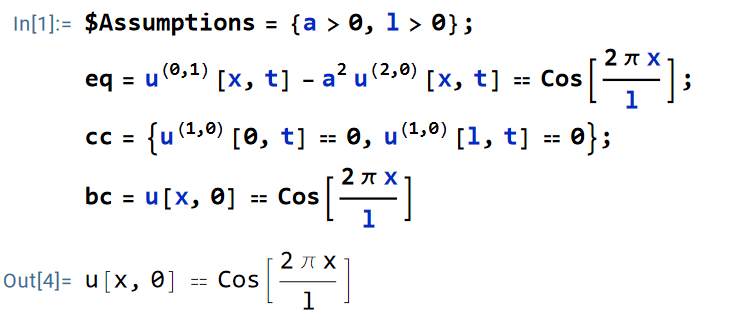
\includegraphics[scale=0.6]{images/img1}
$$
Сперва подставим найденное нами в предыдущем пункте решение для того, чтобы убедиться в правильности:
$$
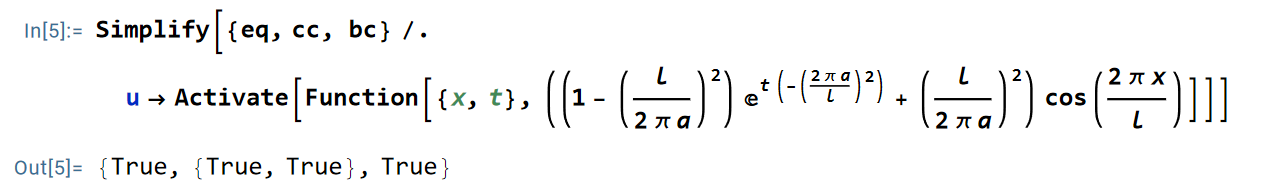
\includegraphics[scale=0.5]{images/img2}
$$
То есть решение было построено верно. Значит найденное с помощью Wolfram Mathematica решение должно совпадать с построенным решением.\\\\
Для получения решения поставленной задачи в Wolfram Mathematica воспользуемся командой DSolve:
$$
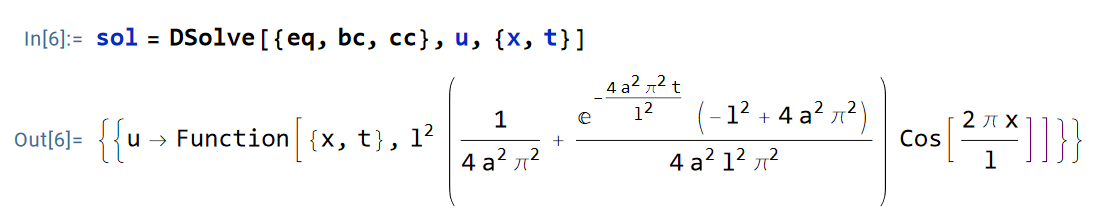
\includegraphics[scale=0.6]{images/img3}
$$
Как можно видеть, мы получили ту же функцию, что и была построена нами аналитически.
\section*{Визуализация решения с помощью Wolfram Mathematica}
Построим интерактивную температурную карту стержня для построенного решения. Для визуализации будем использовать функцию DensityPlot, которая строит
двумерную цветную карту плотностей. По умолчанию цветовая функция
принимает аргументы из отрезка $[0, 1]$, поэтому нужно определить минимум
и максимум функции из начального уравнения исходной задачи
$$
	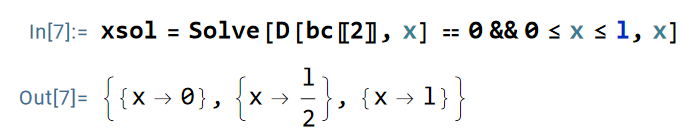
\includegraphics[scale=0.6]{images/img4}
$$
Преобразуем полученный результат в список стационарных точек
$$
	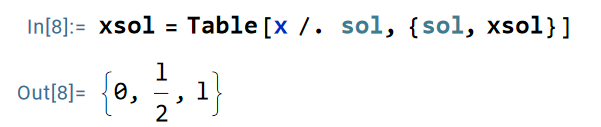
\includegraphics[scale=0.6]{images/img5}
$$
Таким образом, мы имеем список точек, в которых возможны глобальные экстремумы нашей функции. Найдем эти экстремумы:
$$
	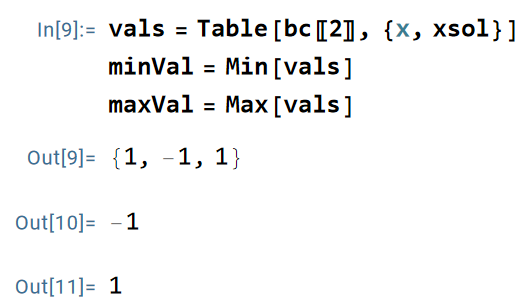
\includegraphics[scale=0.6]{images/img6}
$$
Линейное преобразование, переводящее отрезок [minVal, maxVal] в
отрезок $[0, 1]$, может быть задано в виде анонимной функции следующего вида
$$
	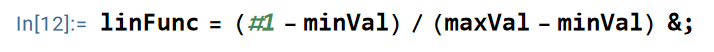
\includegraphics[scale=0.6]{images/img7}
$$
где \#1 -- это первый (для данной функции -- единственный) аргумент анонимной функции.\\\\
Зададим параметры для построения температурной карты:
$$
	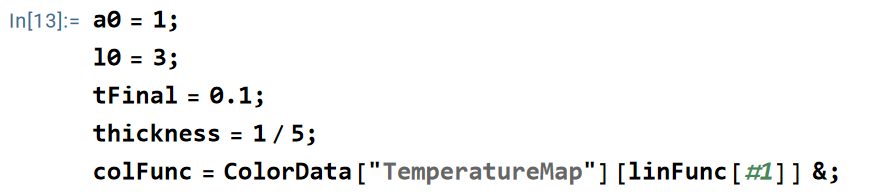
\includegraphics[scale=0.6]{images/img8}
$$
где $a0$, $l0$ -- конкретные значения для параметров $a, l$ исходной задачи, $tFinal$ -- конечный момент времени для интерактивного графика, $thickness$ -- толщина стержня, а функция $colFunc$ будет задавать окраску сечений стержня в зависимости от его температуры в них. TemperatureMap -- это предустановленная в Wolfram Mathematica цветовая схема, в которой нулю (низкая температура) соответствует синий цвет, единице (высокая температура) -- красный.\\\\
Зададим функцию, для которой будет проводиться построение температурной карты, на основе построенного нами решения:
$$
	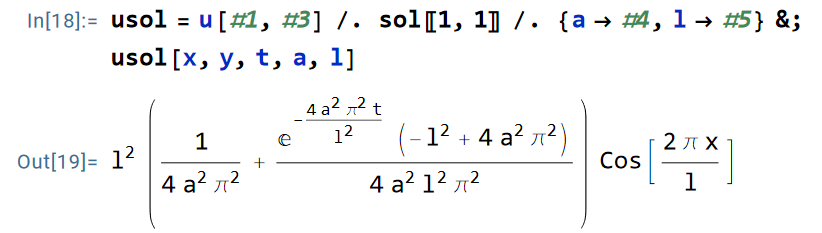
\includegraphics[scale=0.6]{images/img9}
$$
В этой функции параметры $x, t, a, l$ имеют тот же смысл, что и в
исходной задаче, а $y$ -- это координата продольного сечения стержня, которая
является фиктивной. \\\\
Для этой функции построим карту температуры внутри
стержня:
$$
	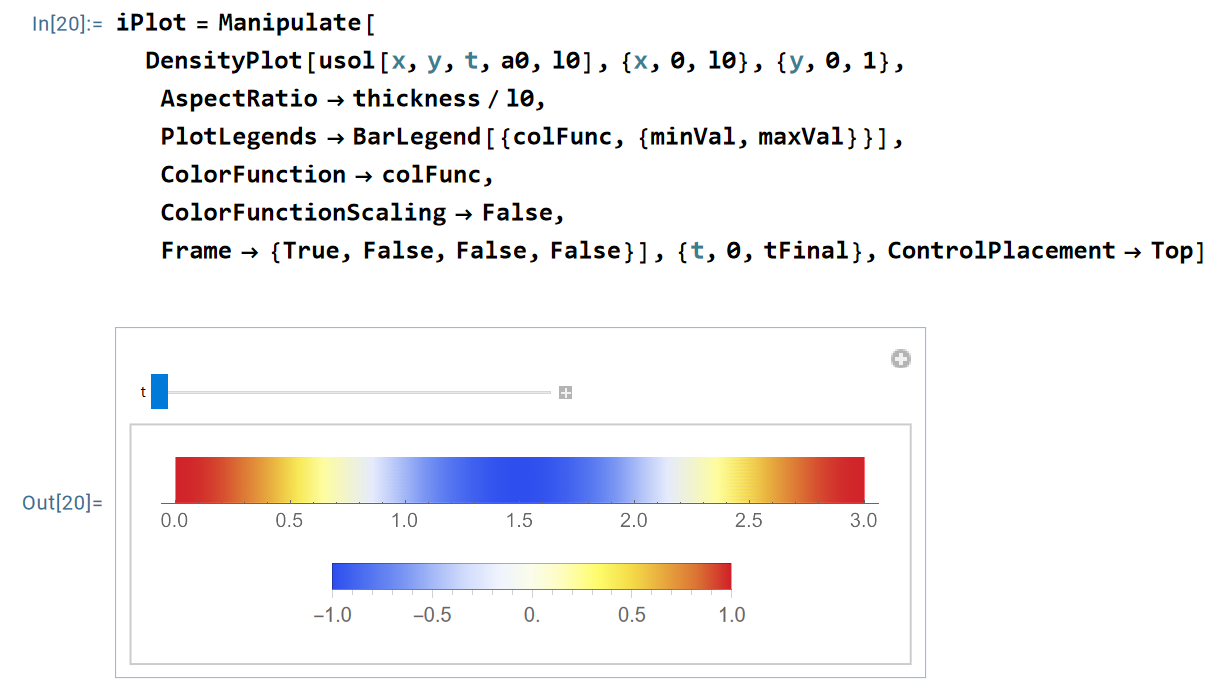
\includegraphics[scale=0.5]{images/img10}
$$
Таким образом, мы построили температурную карту для стержня в момент времени $t = 0$. То есть в начальный момент времени мы имеем максимальную температуру на концах стержня и минимальную в середине. \\\\
При $t=0.09$ карта имеет вид 
$$
	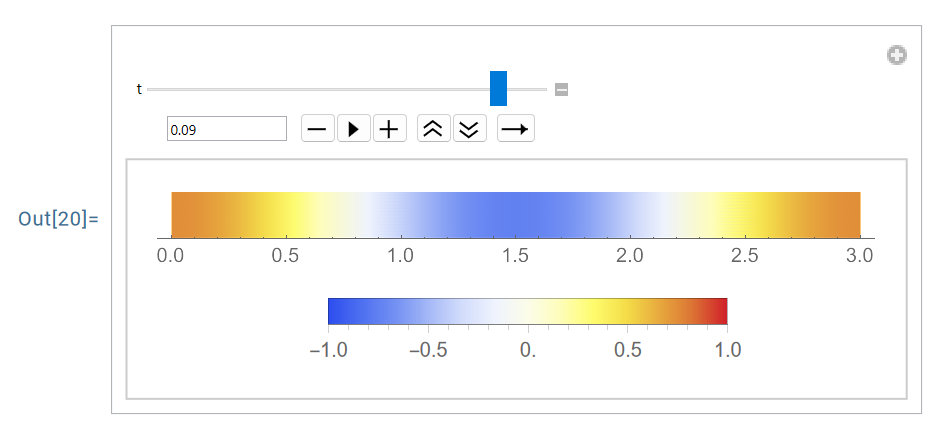
\includegraphics[scale=0.5]{images/img11}
$$
То есть с течением времени температура начинает равномерно распространятся вдоль всего стержня. На концах стержня температура постепенно снижается, а в середине -- повышается.\\\\
Если повысить максимальное значение времени, то, например, в момент времени $t=4$ можно увидеть, что температура вдоль всего стержня близка к средней температуре (между максимальным и минимальным значениями)
$$
	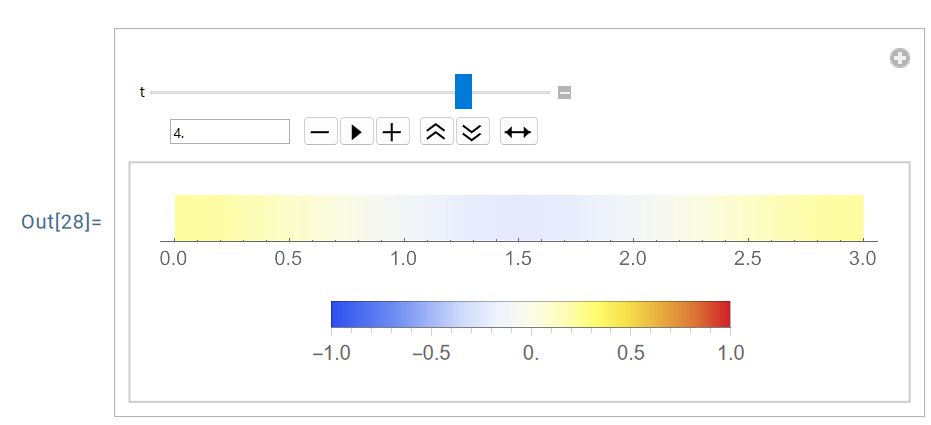
\includegraphics[scale=0.5]{images/img12}
$$
\section*{Вывод}
Таким образом, мы нашли решение смешанной задачи для уравнения теплопроводности методом разделения переменных, а затем проверили, правильно ли оно было вычислено, с помощью Wolfram Mathematica. Для построенного решения мы привели температурную карту, которая при заданных значениях $a, l, t$ и толщины стержня позволяет визуализировать процесс распространения тепла в стержне.
\end{document}

 